% !TEX program = xelatex
\documentclass[12pt]{ctexart}
% ------------------------
% 页面
% ------------------------
\usepackage{geometry}
\geometry{margin=2.5cm}

% ------------------------
% 字体
% ------------------------
\usepackage{fontspec}
\setmainfont{Segoe UI}
\setmonofont{Consolas}

% ------------------------
% 基础包
% ------------------------
\usepackage{multirow}
\usepackage{soul}
\usepackage[normalem]{ulem}
\usepackage{lastpage}
\usepackage{xcolor}
\usepackage{hyperref}
\usepackage{graphicx}
\usepackage{booktabs}
\usepackage{enumitem}
\usepackage{caption}
\usepackage{titlesec}
\usepackage{fancyhdr}
% ------------------------
% GitHub 颜色
% ------------------------
\definecolor{gh-bg}{HTML}{FFFFFF}
\definecolor{gh-border}{HTML}{D0D7DE}
\definecolor{gh-codebg}{HTML}{F6F8FA}
\definecolor{gh-link}{HTML}{0969DA}
\definecolor{gh-line}{HTML}{8B949E}

\definecolor{gh-note}{HTML}{0969DA}
\definecolor{gh-warning}{HTML}{9A6700}
\definecolor{gh-tip}{HTML}{1A7F37}

% ------------------------
% 设置页眉与页尾
% ------------------------
\geometry{left=2cm,right=2cm,top=2cm,bottom=2.5cm}
\fancyhf{}
\fancyhead[C]{}
\fancyhead[L]{中国科学院大学·2026年春}
\fancyhead[R]{网络空间安全导论}
\fancyfoot[C]{第 \thepage 页，共 \pageref{LastPage} 页}
\renewcommand{\footrulewidth}{0.4pt}
\renewcommand{\baselinestretch}{1.2}
\pagestyle{fancy}
% ------------------------
% 超链接
% ------------------------
\hypersetup{
	colorlinks=true,
	linkcolor=gh-link,
	urlcolor=gh-link
}

% ------------------------
% 列表间距
% ------------------------
\setlist{
	itemsep=4pt,
	topsep=6pt
}

% ------------------------
% tcolorbox
% ------------------------
\usepackage{tcolorbox}
\tcbuselibrary{minted,skins,breakable}

% ------------------------
% GitHub 引用块
% ------------------------
\newtcolorbox{ghquote}{
	enhanced,
	colback=white,
	colframe=gh-border,
	borderline west={3pt}{0pt}{gh-border},
	arc=2pt,
	left=10pt,
	right=10pt,
	top=6pt,
	bottom=6pt
}

% ------------------------
% GitHub 提示框
% ------------------------
\newtcolorbox{note}{
	enhanced,
	colback=white,
	colframe=gh-note,
	borderline west={4pt}{0pt}{gh-note},
	title=Note
}

\newtcolorbox{warning}{
	enhanced,
	colback=white,
	colframe=gh-warning,
	borderline west={4pt}{0pt}{gh-warning},
	title=Warning
}

\newtcolorbox{tip}{
	enhanced,
	colback=white,
	colframe=gh-tip,
	borderline west={4pt}{0pt}{gh-tip},
	title=Tip
}

% ------------------------
% 代码块
% ------------------------
\usepackage{minted}

\newtcblisting{codeblock}[2][]{
	listing engine=minted,
	minted language=#2,
	minted options={
		linenos,
		breaklines,
		fontsize=\small,
		numbersep=10pt,
		xleftmargin=15pt
	},
	colback=gh-codebg,
	colframe=gh-border,
	arc=6pt,
	boxrule=0.5pt,
	left=6pt,
	right=6pt,
	top=6pt,
	bottom=6pt,
	listing only,
	breakable,
	#1
}

% ------------------------
% 行内代码
% ------------------------
\newtcbox{\inlinecode}{
	on line,
	boxrule=0pt,
	colback=gh-codebg,
	arc=4pt,
	left=3pt,
	right=3pt,
	top=2pt,
	bottom=2pt
}

% ------------------------
% 标题样式
% ------------------------
\titleformat{\section}
{\Large\bfseries}
{\thesection}{0.5em}{}

\titleformat{\subsection}
{\large\bfseries}
{\thesubsection}{0.5em}{}


\renewcommand{\theFancyVerbLine}{\color{gh-line}\small\arabic{FancyVerbLine}}

\newtheorem{application}{应用}
\newtheorem{problem}{问题}
\newtheorem{analogy}{分析}
\newtheorem{experiment}{实验}

% ------------------------
% 修改表头信息
% ------------------------
%改这里可以修改实验报告表头的信息
\newcommand{\name}{（成员1）陈曦}
\newcommand{\studentNum}{2025K8009970002}
\newcommand{\boxNum}{}
\newcommand{\expNum}{ICS-exp01-01}
\newcommand{\expName}{Linux操作系统的使用与环境搭建}
\newcommand{\finishdate}{2026年3月12日}

% ------------------------
% 文档开始
% ------------------------
\begin{document}
	
	\begin{center}
		\LARGE 中国科学院大学·网络空间安全导论实验报告 
	\end{center}
	
	\begin{center}
		\emph{箱子号} \underline{\makebox[4em][c]{\boxNum}}
		\emph{实验序号} \underline{\makebox[8em][c]{\expNum}}
		\emph{实验专题} \underline{\makebox[16em][c]{\expName}}\\
		\emph{小组成员} \underline{\makebox[36em][c]{\name}}\\
		\emph{对应学号} \underline{\makebox[36em][c]{\studentNum}}\\
		\emph{最后修改日期} \underline{\makebox[34em][c]{\finishdate}}
		{\noindent}
		\rule[8pt]{17cm}{0.2em}
	\end{center}
	\section{摘要}
	本实验采用 WSL2+Ubuntu 搭建环境，旨在掌握 Linux 基础操作、探究核心机制并实现综合应用。完成 10 项基础命令操作，通过 man 手册、跨语言验证及系统测试深入研究了信号机制与命令行参数限制。综合应用 Docker 部署与 Wine 运行，解决了网络超时、依赖缺失等实际问题。借助 AI 工具辅助分析，通过实操验证了 Linux 核心特性，理解了相关工具的实现逻辑，为后续安全实验奠定基础。
	\section{实验环境}
	\begin{enumerate}
		\item[\textbf{1.}]硬件环境
		\begin{center}
			\begin{tabular}{ll}
				\toprule[1pt]
				项目名称 &具体配置\\
				\toprule[1pt]
				设备型号&Lenovo Xiaoxin air15 2020\\
				\midrule
				处理器&AMD Ryzen 7 4800U\\
				\midrule
				内存&16GB（ WSL2 自动管理内存占用）\\
				\midrule
				存储&512GB NVMe 固态硬盘\\
			\end{tabular}
		\end{center}
		\item[\textbf{2.}]软件环境
		\begin{center}
			\begin{tabular}{ll}
				\toprule[1pt]
				项目名称 & 具体配置\\
				\toprule[1pt]
				主操作系统 &Windows 11 家庭版（25H2 内核版本号 26200.7922）\\
				\midrule
				Linux 虚拟化环境 &WSL2（Windows Subsystem for Linux 2，内核版本 5.15.90.1）\\
				\midrule
				Linux 发行版 &Ubuntu 24.04 LTS（64 位）\\
				\midrule
				\multirow{2}{*}{核心工具} &GCC 13.3.0、Python 3.12.3、Vim 9.1、Docker Desktop 4.63.0 (220185)\\
				        &Wine 11.0 Stable、Winetricks 0.0.1-20240105\\
				        \midrule
				辅助工具 &Deepseek R1、浏览器（Microsoft Edge）\\
			\end{tabular}
		\end{center}
	\end{enumerate}
	\section{Linux基本操作实验过程操作步骤}
	\begin{enumerate}
		\item[\textbf{1.}] 构建一个名为\(\,\)\inlinecode{lab1}\(\,\)的文件夹
		\begin{codeblock}{bash}
mkdir lab1
		\end{codeblock}
		\item[\textbf{2.}]进入\(\,\)\inlinecode{lab1}\(\,\)目录\\
		\begin{minipage}{\columnwidth}
			\begin{center}
				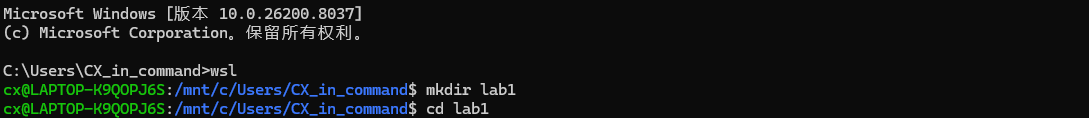
\includegraphics[width=0.8\columnwidth]{pngs/exp1-4.2.png}
				\captionof{figure}{构建并进入文件夹}
			\end{center}
		\end{minipage}
		其中\inlinecode{cd [ DIRECTORY ]}是常用的命令，还有：
		\begin{codeblock}{bash}
cd .   //这里的 .  指代的是当前文件夹
cd ..  //这里的 .. 指代的是父文件夹
cd -   //这里的 -  指代的是上次所访问的目录
cd ~   //这里的 ~  指代的是根目录
		\end{codeblock}
		\item[\textbf{3.}]创建一个C源码，编译并运行一个hello,world：
		\begin{codeblock}{C}
// Hello world的C语言实现:
#include<stdio.h>
int main(){
    printf("Hello,world");
    return 0;
}
		\end{codeblock}
		\begin{minipage}{\columnwidth}
			\begin{center}
				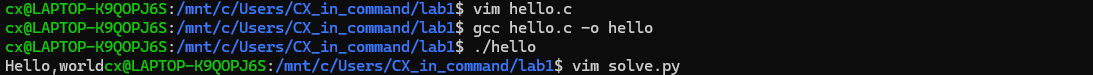
\includegraphics[width=0.8\columnwidth]{pngs/exp1-4.3.png}
				\captionof{figure}{创建Hello，world的C源码，编译运行}
			\end{center}
		\end{minipage}
		\item[\textbf{4.}]用 Python 算第 100 个斐波那契数并存在文件中：
		\par
		\begin{codeblock}{Python}
# 计算斐波那契数列的Python程序实现
def fibonacci(n):
    if n <= 0:
        print("数列index非法")
        return None
    dp = [0] * (n+1)
    dp[0] = 0
    if n >= 1:
        dp[1] = 1
    for i in range(2, n + 1):
        dp[i] = dp[i - 1] + dp[i - 2]
    return dp[n]

if __name__ == "__main__":
    result = fibonacci(100)
    print(result)
		\end{codeblock}
		\begin{minipage}{\columnwidth}
			\begin{center}
				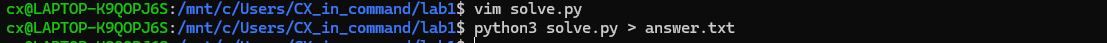
\includegraphics[width=0.8\columnwidth]{pngs/exp1-4.4.png}
				\captionof{figure}{用 Python 算第 100 个斐波那契数并存在文件中}
			\end{center}
		\end{minipage}
		这里解释一下其中的\inlinecode{>}操作符以及一些其他的操作符
		\begin{center}
			\begin{tabular}{ll}
				\toprule
				操作符	&含义\\
				\midrule
				\inlinecode{>}	&写入并覆盖文件\\
				\inlinecode{>>}	&追加写入\\
				\inlinecode{;}	&一行多个的分割符\\
				\bottomrule
			\end{tabular}
		\end{center}
		\item[\textbf{5.}] 拷贝/etc/os-release 文件到当前目录：\\
		\begin{minipage}{\columnwidth}
			\begin{center}
				
\includegraphics[width=0.8\columnwidth]{pngs/exp1-4.5.png}
				\captionof{figure}{拷贝/etc/os-release 文件到当前目录}
			\end{center}
		\end{minipage}
		\item[\textbf{6.}]将/etc/fstab 的 base64 编码写入文件：\\
		\begin{minipage}{\columnwidth}
			\begin{center}
				
\includegraphics[width=0.8\columnwidth]{pngs/exp1-4.6.png}
				\captionof{figure}{将/etc/fstab 的 base64 编码写入文件\(\,\)\inlinecode{fstab\_base64.txt}\(\,\)}
			\end{center}
		\end{minipage}
		\item[\textbf{7.}]查看 /proc/self/maps 并将结果保存到文件中：\\
		\begin{minipage}{\columnwidth}
			\begin{center}
				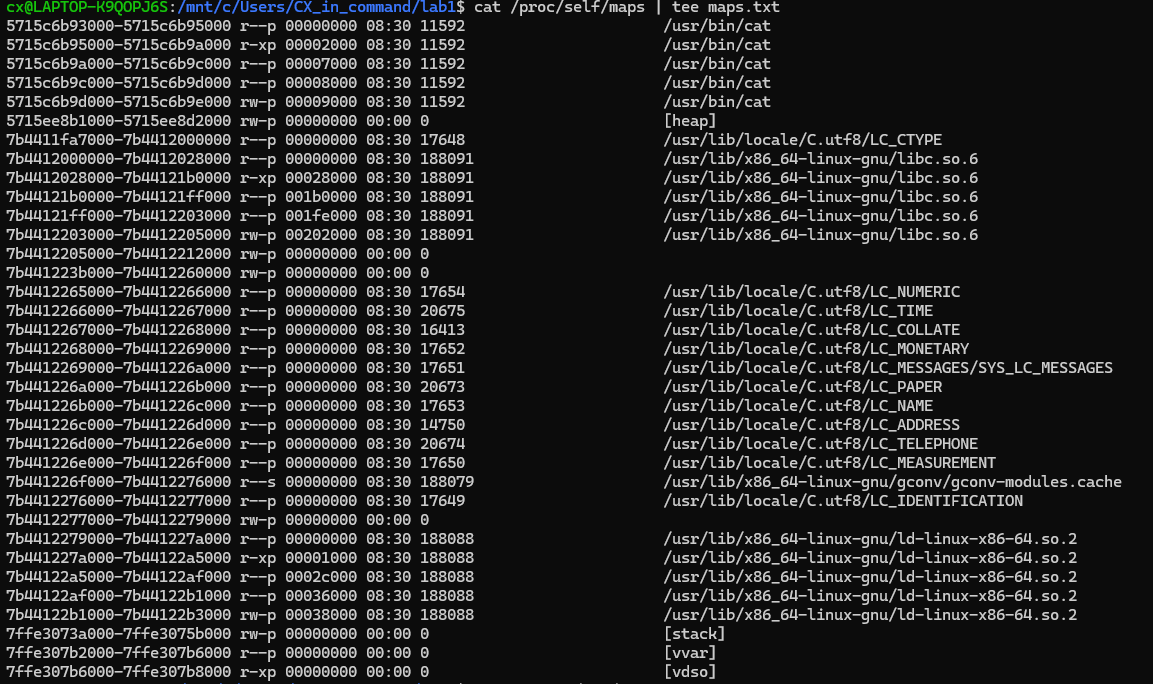
\includegraphics[width=0.8\columnwidth]{pngs/exp1-4.7.png}
				\captionof{figure}{查看 /proc/self/maps 并将结果保存到文件\(\,\)\inlinecode{maps.txt}\(\,\)}
			\end{center}
		\end{minipage}
		这里解释一下Linux操作系统中比较特有的管道操作符 \inlinecode{|}
		
		他允许将前一个命令的输出作为后一个命令的输入
		
		\inlinecode{tee}命令的使用\inlinecode{tee [OPTION] [I/O]}
		\item[\textbf{8.}]将/bin/sh 的十六进制数据存储到文件中：\\
		\begin{minipage}{\columnwidth}
			\begin{center}
				
\includegraphics[width=0.8\columnwidth]{pngs/exp1-4.8.png}
				\captionof{figure}{将/bin/sh 的十六进制数据存储到文件\(\,\)\inlinecode{sh\_hexdump.txt}\(\,\)}
			\end{center}
		\end{minipage}
		\item[\textbf{9.}] 返回上一级目录并打包lab1目录：\\
		这里解释一下tar工具的使用，tar工具(同时配合gzip工具使用)类似于Windows下的\textbf{7-Zip}或者\textbf{WinRAR}，不过相比他们不同的是tar是一个\textbf{命令行应用(CommandLine Application)}。tar工具的使用参数见下表
		\begin{center}
			\begin{tabular}{ll}
				\toprule
				参数&	解释\\
				\midrule
				\inlinecode{-c}	&创建一个归档文件.tar同时配合-f参数使用\\
				\inlinecode{-v}	&显示创建的详细过程\\
				\inlinecode{-z}	&告诉tar创建归档文件的时候要同时压缩\\
				\inlinecode{-r}	&将一个文件添加进这个归档文件.tar中\\
				\inlinecode{-x}	&将一个.tar文件解包成单独的文件\\
				\inlinecode{-C}	&指定解压目录(需要提前创建目录)\\
				\inlinecode{-f}	&指定输出的文件名\\
				\inlinecode{-t}	&列出一个归档包或压缩包的内容\\
				\bottomrule
			\end{tabular}
		\end{center}
		注：tar需要解压的话可以自动识别不需要指定参数\\	
		\begin{minipage}{\columnwidth}
			\begin{center}
				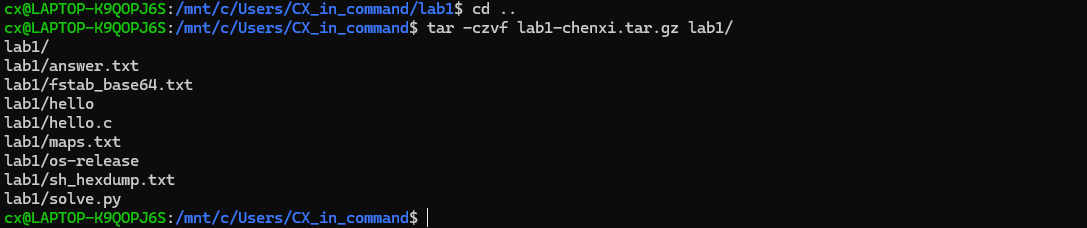
\includegraphics[width=0.8\columnwidth]{pngs/exp1-4.9.png}
				\captionof{figure}{ 返回上一级目录并打包lab1目录}
			\end{center}
		\end{minipage}
	\end{enumerate}
	\section{Linux问题探究}
	\begin{problem}
		Linux 有哪些信号？你可以使用哪些方法来让一个程序（C程序、Python程序、shell程序均可）触发不同的信号？进程收到哪些信号退出时，会在shell中显示进程收到信号的信息？
	\end{problem}
	\begin{analogy}
		研究过程：通过查询网络资料\cite{csdn-signal}与Linux manual(手册)\cite{linux_man}，得知Linux 信号（Signal）是一种 进程间通信（IPC, Inter-Process Communication）机制，用于通知进程某个事件发生。最典型的就是经常在VSCode的控制台中按\(\,\)\inlinecode{Ctrl + C}\(\,\)结束刚编译好的程序\\
		\hspace*{2em}联网搜索得知：通过查阅 \inlinecode{man 7 signal} 文档可以了解到 Linux
		系统中信号（Signal）的类型、默认行为以及信号处理机制。
		需要注意的是，Linux 的 man 手册按章节分类，同一名称
		可能在不同章节中对应不同内容。例如 \inlinecode{man signal}
		通常会打开 signal 系统调用或库函数的说明，而
		\inlinecode{man 7 signal} 则提供了 Linux 信号机制的总体介绍。\\
		\begin{minipage}{\columnwidth}
			\begin{center}
				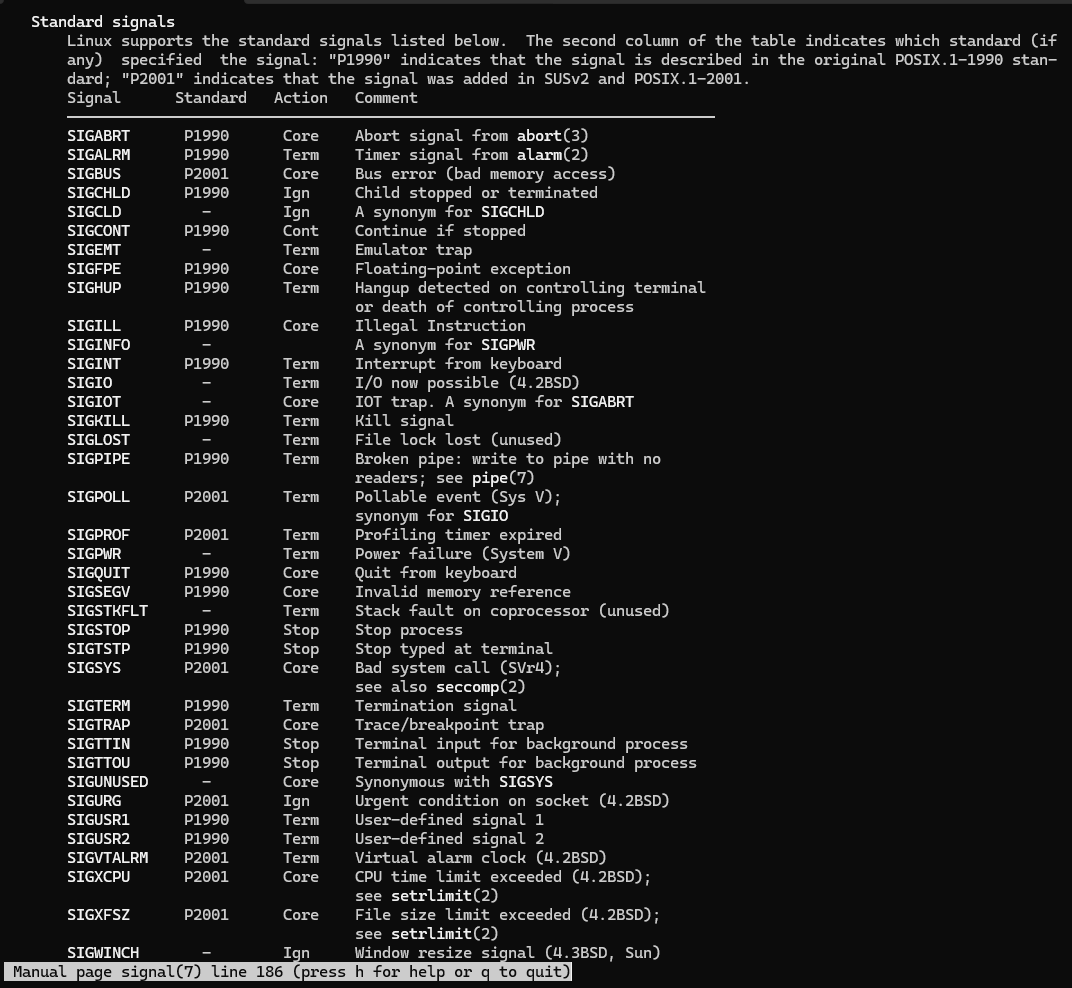
\includegraphics[width=0.6\columnwidth]{pngs/man_7_signal.png}
				\captionof{figure}{列出Linux中所有信号}
			\end{center}
		\end{minipage}
		\hspace*{2em}同时使用\(\,\)\inlinecode{man signal}\(\,\)我们可以看到Linux系统下程序如何使用 signal 相关函数处理信号\\
		\begin{minipage}{\columnwidth}
			\begin{center}
				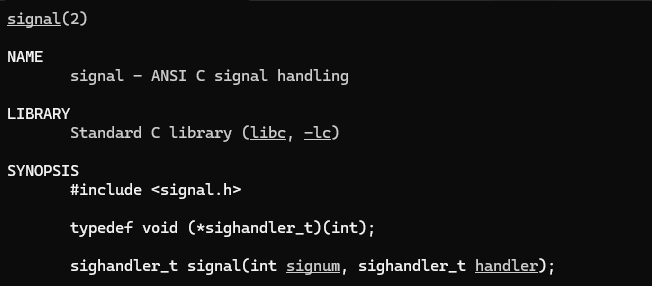
\includegraphics[width=0.5\columnwidth]{pngs/man_signal.png}
				\captionof{figure}{Linux系统中对Signal的C标准库的说明}
			\end{center}
		\end{minipage}
		\hspace*{2em}很自然的，我们会想到C程序的信号触发方式，
		\begin{codeblock}{C}
// 5 秒后程序给自己发送 SIGINT
#include <signal.h>
#include <stdio.h>
#include <unistd.h>
int main(){
    printf("PID = %d \n", getpid());
    sleep(5);
    raise(SIGINT);
    printf("If this program were still running, it would print this message.\n");
    return 0;
}
		\end{codeblock}
		运行如下\\
		\begin{minipage}{\columnwidth}
			\begin{center}
				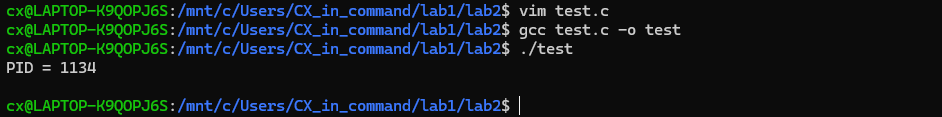
\includegraphics[width=0.5\columnwidth]{pngs/signal_c.png}
				\captionof{figure}{C程序触发信号SIGINT(类似于\(\,\)\inlinecode{Ctrl + C}\(\.\))}
			\end{center}
		\end{minipage}
		\hspace*{2em}除了程序触发外，还有手动输入的方式如:\\
		 	 \hspace*{2em}·Ctrl + C\(\,\)触发SIGINT\\
		 	 \hspace*{2em}·Ctrl + \textbackslash \(\,\)触发SIGQUIT\\
		 	 \hspace*{2em}·Ctrl + Z\(\,\)触发SIGTSTP\\
		 \hspace*{2em}同时还有一种内核在检测到异常或错误时抛出 Signal(比如检测到除以零，或者是某些I/O异常)\\
		\hspace*{2em}另外，当程序因为 信号终止，shell 有时会显示提示。例如：
		\begin{codeblock}{sh}
Segmentation fault (core dumped)  
		\end{codeblock}
		常见情况：
		\begin{center}
			\begin{tabular}{ll}
				\toprule
				信号	&shell显示\\
				\midrule
				SIGSEGV	&Segmentation fault\\
				SIGABRT	&Aborted\\
				SIGFPE	&Floating point exception\\
				SIGILL	&Illegal instruction\\
				SIGQUIT	&Quit\\
				SIGPIPE	&Broken pipe\\
				\bottomrule
			\end{tabular}
		\end{center}
		\hspace*{2em}例子：
		\begin{codeblock}{C}
// C程序触发信号SIGSEGV，shell显示提示
#include <stdio.h>
int main(){
    int *p = NULL;
    *p = 5;
}
		\end{codeblock}
		运行如下：\\
		\begin{minipage}{\columnwidth}
			\begin{center}
				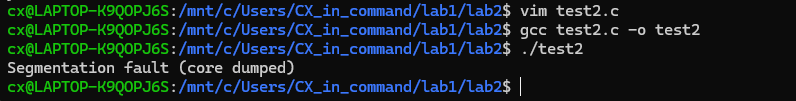
\includegraphics[width=0.5\columnwidth]{pngs/coredumped.png}
				\captionof{figure}{C程序触发信号SIGSEGV，shell显示提示}
			\end{center}
		\end{minipage}
		\textbf{实验结论}
		\begin{itemize}
			\item Linux 信号是进程间通信机制之一。
			\item 可以通过 kill、键盘、系统调用触发信号。
			\item 不同信号默认行为不同。
			\item 当程序因异常信号退出时，shell 会输出错误信息。
		\end{itemize}
	\end{analogy}
	\begin{problem}
		一个程序的命令行参数是什么？有什么限制？它在一个程序（C程序、Python程序、shell程序均可）中是如何使用的？
	\end{problem}
	\begin{analogy}
		这一点可以从我们日常使用的命令行工具找到答案。例如我们常使用的
		\begin{codeblock}{sh}
ls -l /home
		\end{codeblock}
		其中的\(\,\)\inlinecode{-l~ /home}\(\,\)部分称作命令行参数，相当于将程序的Input前置。对于Linux系统原生支持的C语言而言，命令行参数在于\(\,\)\inlinecode{main()}\(\,\)函数的可选参数中
		\begin{codeblock}{C}
int main(int argc, char *argv[]) 
// 在许多古早的代码如ls工具中也写成
int main(int argc, char **argv)
		\end{codeblock}
		\begin{center}
			\begin{tabular}{ll}
				\toprule
				参数	&含义\\
				\midrule
				argc&	参数数量\\
				argv&	参数字符串数组\\
				\bottomrule
			\end{tabular}
		\end{center}
		\hspace*{2em}示例程序：
		
		\begin{codeblock}{C}
#include<stdio.h>
int main(int argc, char *argv[]){
    printf("argc = %d\n", argc);
    for(int i = 0; i < argc; i++){
        printf("argv[%d] = %s\n", i, argv[i]);
    }
    return 0;
}
		\end{codeblock}
		\begin{minipage}{\columnwidth}
			\begin{center}
				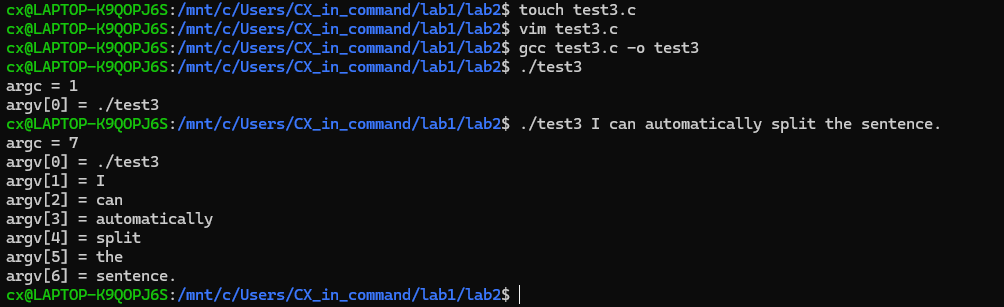
\includegraphics[width=0.5\columnwidth]{pngs/parameter.png}
				\captionof{figure}{获取命令行参数}
			\end{center}
		\end{minipage}
		\hspace*{2em}其中 \texttt{argv[0]} 通常表示程序自身的名称。剩下的从\(\,\)\inlinecode{1 -> argc-1}\(\,\)都是OS主动将参数以空格拆分得到的多个字符串\\
		\textbf{而对于其他语言：}\\
		\hspace*{2em}在 Python 中可以通过 \texttt{sys.argv} 获取命令行参数。\\
		\hspace*{2em}示例代码：
		\begin{codeblock}{python}
import sys

if __name__ == "__main__":
    print(len(sys.argv))
    for arg in sys.argv:
        print(arg)
		\end{codeblock}
		运行示例：\\
		\begin{minipage}{\columnwidth}
			\begin{center}
				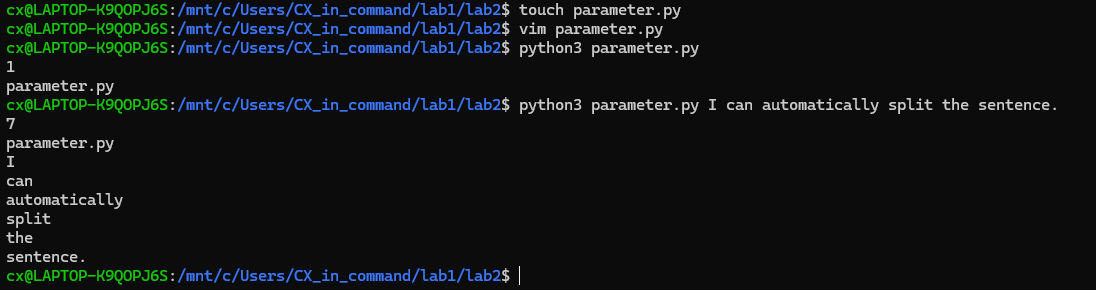
\includegraphics[width=0.5\columnwidth]{pngs/py_parameter.png}
				\captionof{figure}{Python程序获取命令行参数}
			\end{center}
		\end{minipage}
		\hspace*{2em}在 Shell 脚本中，命令行参数可以通过 \inlinecode{\$1}、\inlinecode{\$2} 等变量访问，\inlinecode{\$\#} 表示参数数量。\\
		\hspace*{2em}示例脚本：
		\begin{codeblock}{bash}
#!/bin/bash
echo "first argument: $1"
echo "second argument: $2"
echo "number of arguments: $#"
		\end{codeblock}
		
		运行示例：\\
		\begin{minipage}{\columnwidth}
			\begin{center}
				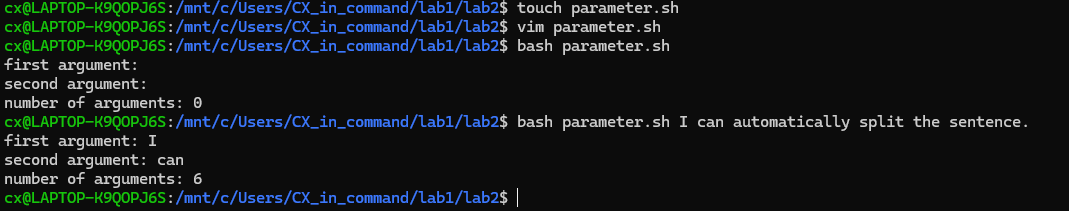
\includegraphics[width=0.5\columnwidth]{pngs/bash_parameter.png}
				\captionof{figure}{Shell脚本获取命令行参数}
			\end{center}
		\end{minipage}
		\hspace*{2em}而这项功能的最大作用就是开发所谓的命令行式应用（Command-Line Application）。这种应用没有GUI(图形界面)，资源占用少，效率高；通过解析不同组合的参数实现特定的功能。或者某种意义上也叫做脚本\\
		\hspace*{2em}而当然，对于这种C风味的字符串数组，一般都有一个固定的上限长度。该限制由内核参数 \inlinecode{ARG\_MAX} 决定。可以通过以下命令查看该限制：
		\begin{codeblock}{sh}
getconf ARG_MAX
		\end{codeblock}
		在实验环境中得到的结果为：\\
		\begin{minipage}{\columnwidth}
			\begin{center}
				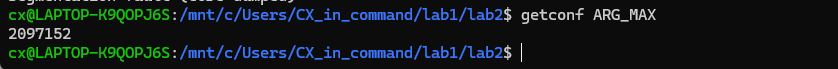
\includegraphics[width=0.5\columnwidth]{pngs/ARG_MAX.png}
				\captionof{figure}{实验室得到的ARG\_MAX参数}
			\end{center}
		\end{minipage}
		\hspace*{2em}同时我们使用shell命令构造超长参数，此时内核拒绝创建新进程，内核抛出错误：\\
		\begin{minipage}{\columnwidth}
			\begin{center}
				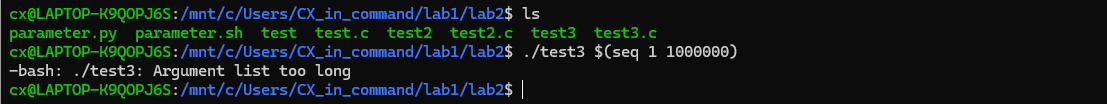
\includegraphics[width=0.5\columnwidth]{pngs/ultrallong-parameters.png}
				\captionof{figure}{命令行参数超过ARG\_MAX时}
			\end{center}
		\end{minipage}
		\textbf{实验总结}\\
		\hspace*{2em}命令行参数是程序启动时从命令行传入的参数，用于控制程序的运行行为。\\
		\hspace*{2em}在不同语言中访问命令行参数的方法不同：
		
		\begin{itemize}
			\item C 语言：通过 \inlinecode{argc} 和 \inlinecode{argv}
			\item Python：通过 \inlinecode{sys.argv}
			\item Shell：通过 \inlinecode{\$1}、\inlinecode{\$2} 等变量访问参数值，\inlinecode{\$\#} 访问参数数量
		\end{itemize}
		
		同时，Linux 系统对命令行参数的总长度存在限制，该限制由系统参数
		\(\,\)\inlinecode{ARG\_MAX}\(\.\) 决定。
	\end{analogy}
	\section{Linux综合应用}
	\begin{application}
		安装 Docker 并运行 Hello World
	\end{application}
	\begin{experiment}
		首先，由于我使用的是WSL2的环境，考虑到希望同时在主机Windows系统及多个WSL的容器中方便地使用Docker，因此选择在主机Windows系统上安装Docker Desktop应用，通过挂载的方式分配给Linux虚拟机使用。首先安装Docker Desktop.之后全程采用GUI操作，十分方便(\sout{PS:我这是不是算走捷径})\\
		\hspace*{2em}然后启动应用，来到\(\,\)\inlinecode{Setting \(\to\) Resources \(\to\) WSL Integration }\(\,\)此处，勾选启用Docker与WSL的集成，并选择需要启用Docker的特定Linux发行版。\\
		\begin{minipage}{\columnwidth}
			\begin{center}
				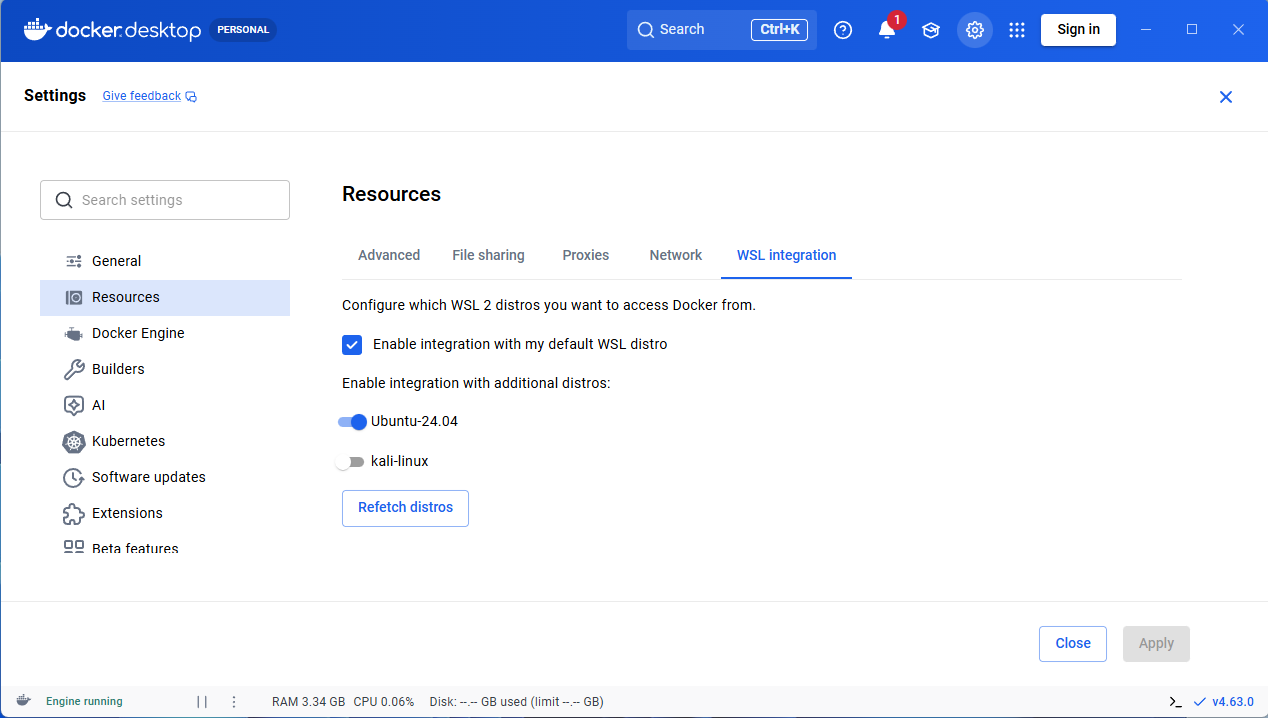
\includegraphics[width=0.5\columnwidth]{pngs/docker_wsl.png}
				\captionof{figure}{为WSL启用Docker}
			\end{center}
		\end{minipage}
		\hspace*{2em}此时，Docker自动配置完成，在WSL的Ubuntu系统的Bash中输入
		\begin{codeblock}{bash}
docker version
		\end{codeblock}
		Shell输出提示：\\
		\begin{minipage}{\columnwidth}
			\begin{center}
				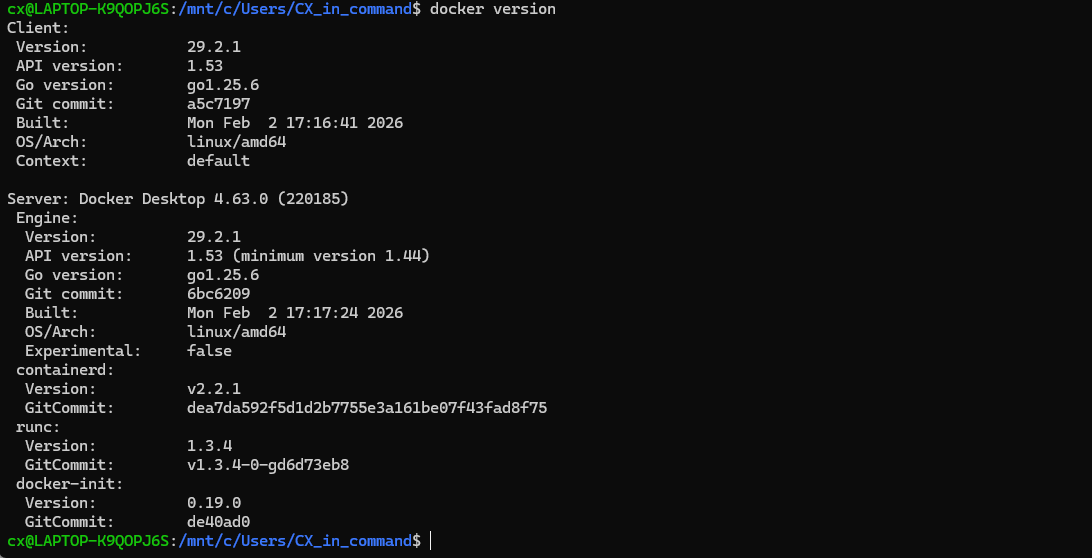
\includegraphics[width=0.4\columnwidth]{pngs/docker_version.png}
				\captionof{figure}{在Shell中输入docker version}
			\end{center}
		\end{minipage}
		\hspace*{2em}然后开始访问Docker Hub下载官方的hello-world容器运行。但是第一次运行时发现，Shell界面长时间未响应，因此选择\inlinecode{Ctrl + C}退出。\\
		\begin{minipage}{\columnwidth}
			\begin{center}
				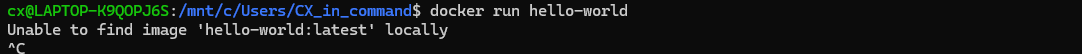
\includegraphics[width=0.5\columnwidth]{pngs/dockertimeout.png}
				\captionof{figure}{下载hello-world容器但长时间未响应}
			\end{center}
		\end{minipage}
		\hspace*{2em}\hyperlink{systemctl}{参考AI辅助分析}，尝试运行
		\begin{codeblock}{sh}
systemctl status docker
		\end{codeblock}
		检查docker守护进程运行状态，是不是Docker进程被kill掉了，但是提示\inlinecode{docker.service Not Found}\\
		\begin{minipage}{\columnwidth}
			\begin{center}
				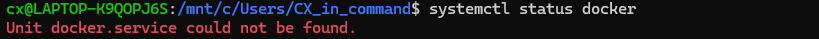
\includegraphics[width=0.5\columnwidth]{pngs/systemctl.png}
				\captionof{figure}{查询Docker守护进程状态}
			\end{center}
		\end{minipage}
		 \hspace*{2em}分析本机安装的特殊性发现：本机Docker的主进程事实上是在Windows上的，Linux上的只是一个挂载的Docker套皮。所以\inlinecode{systemd}事实上不会管理到本机的docker程序。也就是说问题的根源还是在网络上。受到GFW(Great Firewall)影响，从国内访问国外的Docker Hub网站下载容器几乎是被阻塞的，所以需要一些"魔法科技"("梯子")。挂上"梯子"之后，就成功从Docker Hub上下载并成功运行了官方的hello-world容器，同时产生了合适的输出了\\
		\begin{minipage}{\columnwidth}
			\begin{center}
				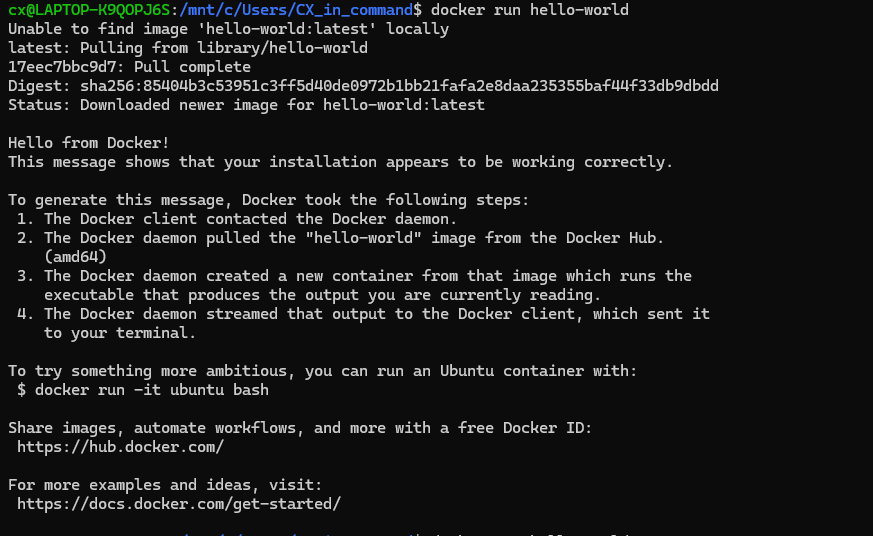
\includegraphics[width=0.5\columnwidth]{pngs/docker_hello-world.png}
				\captionof{figure}{运行hello-world容器}
			\end{center}
		\end{minipage}
		
		\textbf{对Docker的理解：不只是虚拟化}\\
		\hspace*{2em}说实话，在动手安装之前，我以为 Docker 就和平时用的虚拟机差不多：装一个系统环境，在里面跑应用。但Docker事实上比我想象的要“轻”得多——与其说是虚拟机，Docker 更像是对Linux操作系统内核功能的二次封装。
		
		具体来说，Linux 内核早就支持把进程隔离开，还能限制每个进程对 CPU、内存的占用。这些功能以前是给系统管理员做高级调优用的，但 Docker 把它们用起来了：每一个容器其实就是一个被“隔离”起来的普通进程，它有自己的文件系统、网络、进程编号，但用的还是同一个 Linux 内核。所以容器启动特别快，占用的资源也少，不像虚拟机还要模拟一整台电脑。
		
		Docker 通过对运行环境的打包，实现了 ‘一次构建，随处运行’。从某种视角看，它和 JVM 都提供了\textbf{环境抽象}：JVM 抽象了操作系统和硬件，让 Java 程序跨平台运行；而 Docker 抽象了操作系统发行版和依赖，让应用容器能在不同 Linux 环境下一致运行。虽然两者的实现原理完全不同：JVM 是语言虚拟机，Docker 是操作系统级虚拟化，直接使用宿主机内核。
	\end{experiment}
	\begin{application}
		使用 Wine 运行 Windows 程序
	\end{application}
	\begin{experiment}
		参考知乎Linux中国的解释文档：\cite{linux-zhihu}\href{https://zhuanlan.zhihu.com/p/645456382}{如何在 Ubuntu 中安装 Wine | Linux 中国}\\
		同时参考另一个CSDN Blog文档：\cite{wine-csdn}\href{https://blog.csdn.net/XiaoYuHaoAiMin/article/details/141901660}{Ubuntu24使用Wine运行Windows程序安装微信}
		\begin{itemize}
		\item 选择从wine的存储库安装最新的版本
		\begin{enumerate}
			\item 首先输入下面的代码使得在我的发行版上添加 32 位架构的支持
			\begin{codeblock}{bash}
sudo dpkg --add-architecture i386
			\end{codeblock}
			\item 下载和添加存储库密钥:
			\begin{codeblock}{bash}
sudo mkdir -pm755 /etc/apt/keyrings
sudo wget -O /etc/apt/keyrings/winehq-archive.key https://dl.winehq.org/wine-builds/winehq.key
			\end{codeblock}
			\item 现在，下载 WineHQ 源文件文件。由于我使用的Linux发行版是Ubuntu-24.04，此时参考CSDN Blog中的添加方式：(注意不同的Ubuntu版本对应的 winehq-代号 不同，不可以随意使用)
			\begin{codeblock}{bash}
sudo wget -NP /etc/apt/sources.list.d/ https://dl.winehq.org/wine-builds/ubuntu/dists/noble/winehq-noble.sources
			\end{codeblock}
			在完成后，更新软件包信息(\textbf{必须要干})和安装 Wine 的稳定版本软件包。
			\begin{codeblock}{bash}
sudo apt update
sudo apt install --install-recommends winehq-stable
			\end{codeblock}
			安装Wine的辅助工具Winetricks：
			\begin{codeblock}
sudo apt install winetricks
			\end{codeblock}
		\end{enumerate}
		\item 初始化 Wine 配置\\
		\hspace*{2em}初始化wine环境，使用以下命令安装wine-mono组件来支持.NET应用：
		\begin{codeblock}{bash}
winecfg
		\end{codeblock}
		\hspace*{2em}使用Winetricks检查wine-mono和wine-gecko是否安装成功，执行如下命令，然后依次选择\(\,\)\inlinecode{选择默认的wine容器 $\to$ 运行卸载程序}，在弹出的窗口中如果发现了wine-mono和wine-gecko，则说明wine-mono和wine-gecko安装成功。：
		\begin{codeblock}{bash}
winetricks
		\end{codeblock}
		\begin{minipage}{\linewidth}
			\begin{center}
				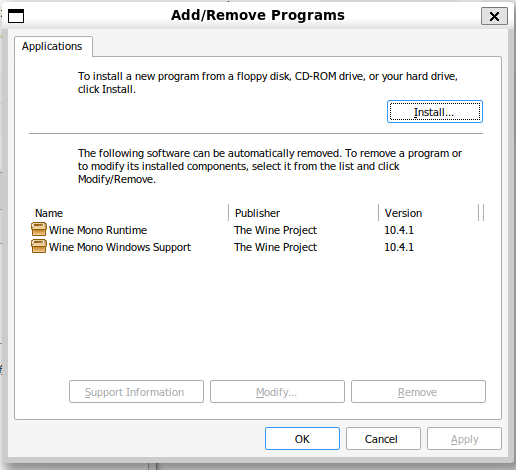
\includegraphics[width=0.3\columnwidth]{pngs/winetricks.png}
				\captionof{figure}{使用winetricks检查自动安装程序有无安装上面两个程序}
			\end{center}
		\end{minipage}
		\hspace*{2em}发现仍然缺少wine-gecko，下面进入清华开源下载站下载。打开清华大学开源软件镜像站wine-gecko目录：\href{https://mirrors.tuna.tsinghua.edu.cn/winehq/wine/wine-gecko/}{清华下载站下载}，找到最新版wine-gecko（非rc版），下载其msi格式的安装包（需要下两个，32位x86的和64位x86\_64的）：下载好后打开winetricks，然后选择上图中的Install选项选中对应的.msi程序安装，等待一段时间后安装完成\\
		\begin{minipage}{\linewidth}
			\begin{center}
				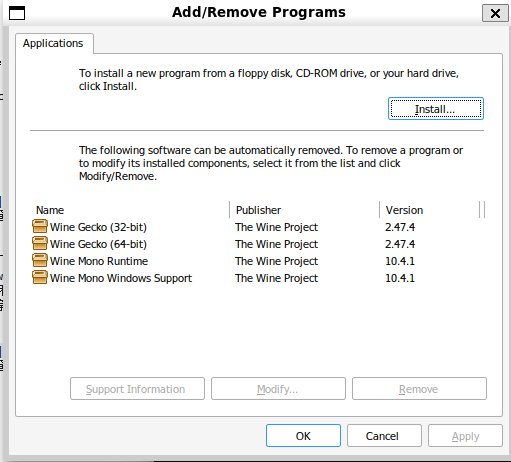
\includegraphics[width=0.3\columnwidth]{pngs/winetricksok.png}
				\captionof{figure}{使用winetricks检查wine-gecko是否安装完整}
			\end{center}
		\end{minipage}
		\item \textbf{安装常用配置}\\
		\hspace*{2em}安装常用字体，输入下列命令：
		\begin{codeblock}{bash}
winetricks allfonts corefonts cjkfonts
		\end{codeblock}
		\hspace*{2em}安装DirectX提升兼容性和应用性能
		\begin{codeblock}{bash}
winetricks d3dx9 d3dx10
		\end{codeblock}
		\hspace*{2em}安装 VC++2022 运行库
		\begin{codeblock}{bash}
winetricks vcrun2022
		\end{codeblock}
		
		\item 下面以7-Zip为例子来展示wine的使用：\\
		\begin{minipage}{\linewidth}
			\begin{center}
				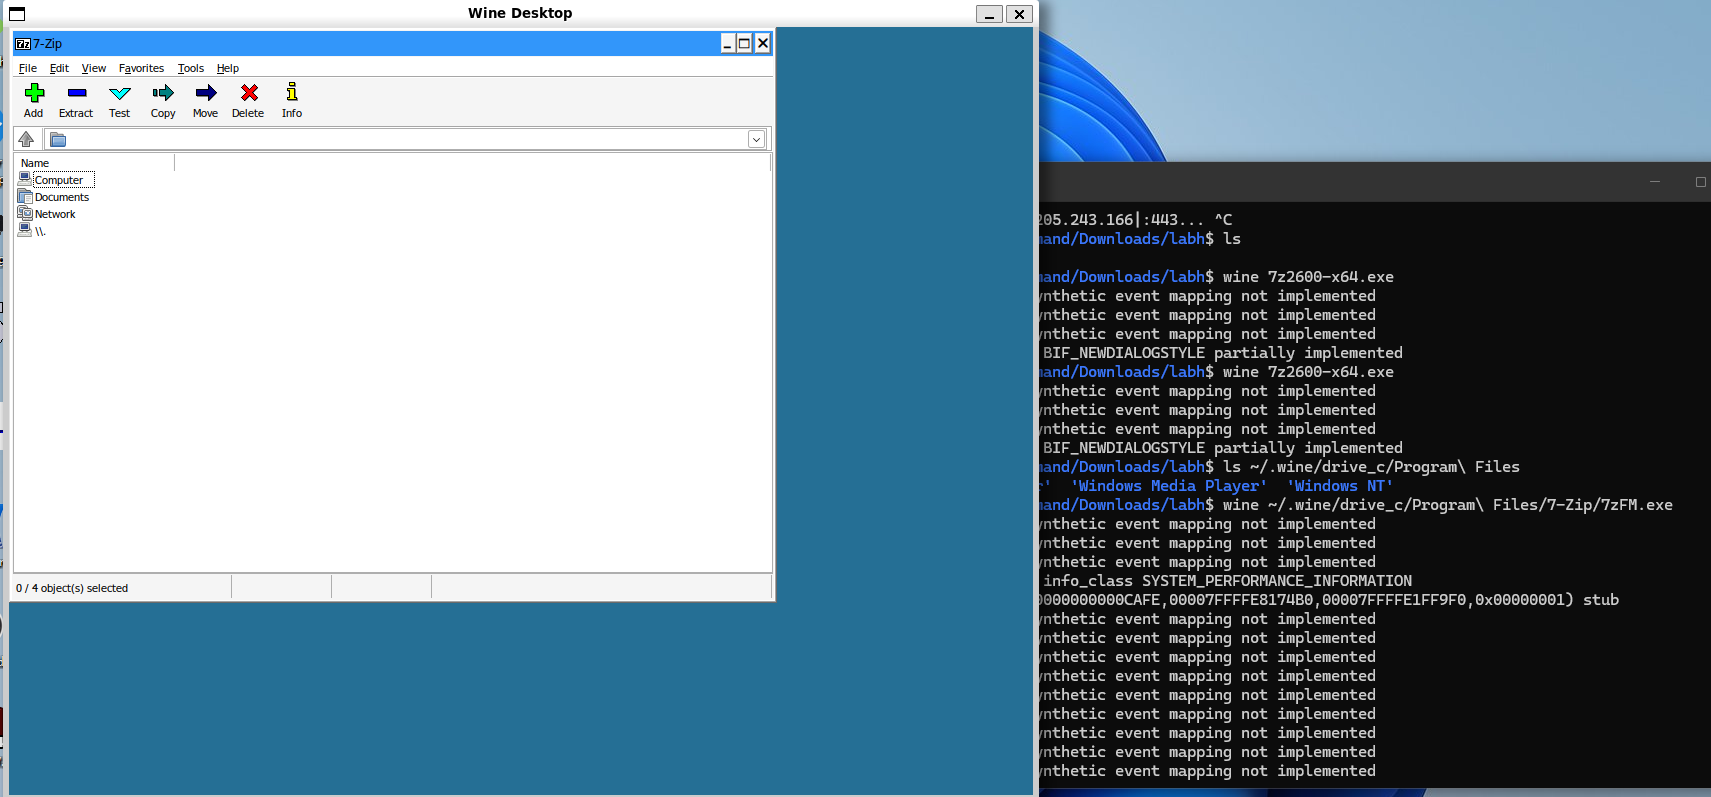
\includegraphics[width=\columnwidth]{pngs/7-zip.png}
				\captionof{figure}{使用wine启动7-Zip}
			\end{center}
		\end{minipage}
		
	\end{itemize}
	\textbf{实验总结}\\
	\hspace*{2em}通过本实验，我在 Linux 环境中成功安装并配置了 Wine，并使用 Wine 成功运行了 Windows 程序。实验过程中，我了解了 Wine 的工作原理:
	\begin{note}
		即通过实现 Windows API 接口，使 Windows 应用程序能够在 Linux 系统上运行，而无需安装完整的 Windows 操作系统。
	\end{note}
	相比虚拟机方案，Wine 具有资源消耗低、运行效率高等优势，但其兼容性仍然有限，一些复杂的 Windows 程序可能无法正常运行。总体而言，Wine 是一种轻量级且高效的跨平台解决方案，在 Linux 环境中运行 Windows 应用具有重要意义。
	\end{experiment}
	\section{参考文献与附录}
	\begin{thebibliography}{9}
		\bibitem{csdn-signal}
		Linux--信号（万字详解！超完整！） [N]\href{https://blog.csdn.net/2301\_76618602/article/details/139576092}{https://blog.csdn.net/2301\_76618602/article/details/139576092}
		\bibitem{linux_man}
		Linux man-pages project. (2023). \textit{signal(7) — Linux manual page}.
		\bibitem{linux-zhihu}
		如何在 Ubuntu 中安装 Wine | Linux 中国 [N] \href{https://zhuanlan.zhihu.com/p/645456382}{https://zhuanlan.zhihu.com/p/645456382}
		\bibitem{wine-csdn}
		Ubuntu24使用Wine运行Windows程序安装微信 [N] \\
		\href{https://blog.csdn.net/XiaoYuHaoAiMin/article/details/141901660}{https://blog.csdn.net/XiaoYuHaoAiMin/article/details/141901660}
	\end{thebibliography}
	\textbf{AI辅助呈现}\\
	\begin{minipage}{\linewidth}
		\begin{center}
			\hypertarget{systemctl}{}
			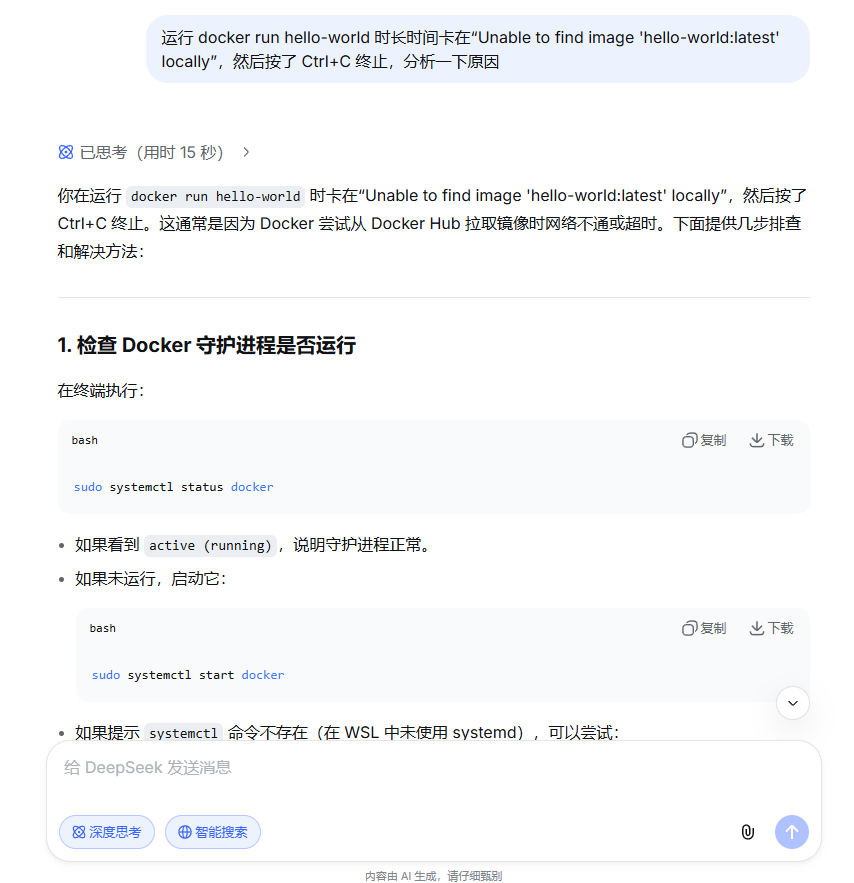
\includegraphics[width=\columnwidth]{pngs/deepseekr1.png}
		\end{center}
	\end{minipage}
		
\end{document}